%% ----------------------------------------------------------------
%% RetinaNet.tex
%% ---------------------------------------------------------------- 
\chapter{RetinaNet} \label{Chapter:RetinaNet}

This chapter introduces RetinaNet \cite{lin2017focal}, a single-stage framework that achieves state-of-the-art performance and high detection rates; it also provides information about technical specifications and the concepts met in every object detector in a more detailed manner. 

\section{Prior Bounding Boxes (Anchors)}\label{anchor_box}
Anchors act as reference boxes around RoIs, in order to get refined later from the regressor head. Instead of producing new coordinates for every detection, predicting the offsets $(\Delta x, \Delta y, \Delta w, \Delta h)$ of a predefined bounding box is much more efficient. Anchor boxes can be more than one, of different scales and ratios depending on the variance of the dataset (e.g. for pedestrian detection, an elongated anchor box would be more useful than a square one).

Usually, most models define by default 9 anchor boxes with scales of $(2^0, 2^{1/3}, 2^{2/3})$ and ratios of $(1\!:\!2,1\!:\!1,2\!:\!1)$, but this depends on the variation of the objects in the dataset. K-means clustering over the dataset is a common method to find the most representatives scales and ratios.

\fref{ch3:fig1} shows an $8\times8$ feature map where each grid cell tries to optimally fit nine anchor boxes of area $K\times K$. Each grid cell represents a spatial area of $(\frac{W}{8}, \frac{H}{8})$ in the original image. The cell in $(3,3)$ makes a positive detection if $p(obj)$ is bigger than a certain threshold. The proposed prediction from this cell, will be the anchor with the highest $p(obj)$. The nearest potential prediction's centre would have at least 8 pixels distance from the previous on any adjacent cell; therefore, this feature map's predictions are characterised by a stride = 8. Feature maps of bigger spatial size can achieve more dense predictions. Precisely, stride has a direct relationship with the number of pooling layers and equals to the total number of times the feature map has been downsampled from the original image.

 \begin{figure}[!htb]
  \centering
  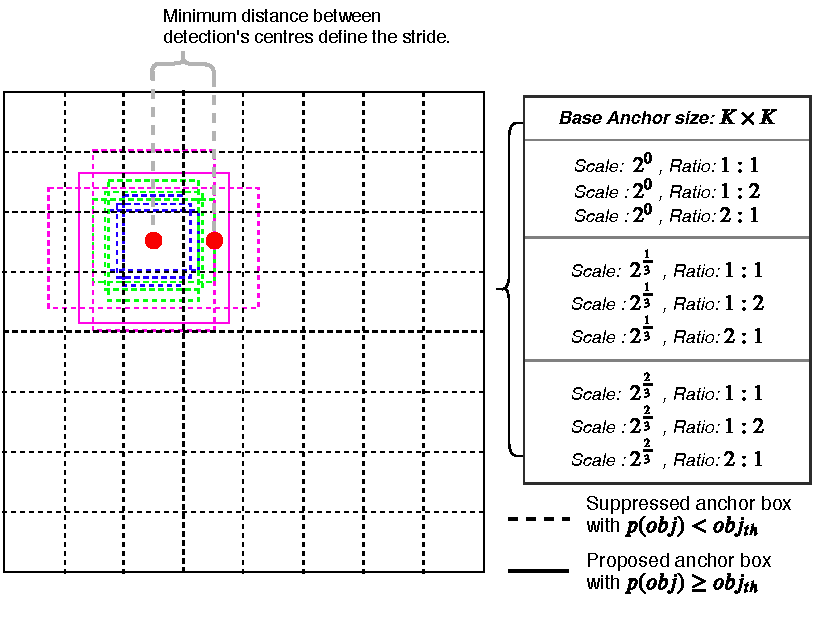
\includegraphics[width=7cm]{figures/ch3/fig1.pdf}
  \caption{A typical topology with 9 anchors acting as prior bounding boxes. Larger feature maps make denser predictions due to their small stride.}
  \label{ch3:fig1}
\end{figure} 

To associate ground truth boxes with suitable anchors, each anchor gets assigned with the overlap between the anchor box and the ground truth box (if any). If the IoU overlap is more than 0.5, then this anchor should be proposed for detection, and it is called a \textbf{\textit{positive anchor}}. If the IoU overlap is less than 0.4, that anchor is going to get suppressed, and it is classified as a \textbf{\textit{negative anchor}}. During training, if an anchor is neither positive nor negative, it does not contribute to the overall loss.

\section{Intersection Over Union}
Intersection over Union (IoU), or Jaccard index, is an evaluation metric used to measure how accurately a predicted box matches or overlaps the ground truth box. As the name indicates, IoU is the ratio between the intersection and the union of two boxes. In most tasks, as in PASCAL-VOC challenge, if the IoU between the detection and the ground truth is more than 0.5, the detection counts as a true positive.

\begin{figure}[!b]
  \centering
  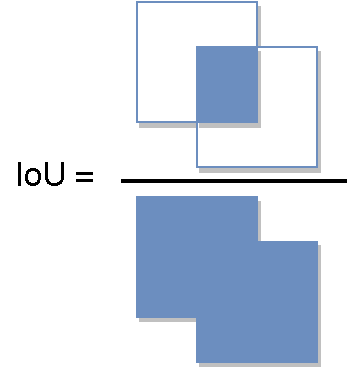
\includegraphics[width=0.25\textwidth]{figures/ch3/fig2.pdf}
  \caption{The Intersection over Union ratio is a widely adopted metric to measure bounding boxes' overlap.}
  \label{ch3:fig2}
\end{figure} 

\section{Non-Maximum Suppression}
Usually, objects extend much more in space rather than occupying only a grid cell on the feature map. Thus, many adjacent grid cells, by processing similar context of information, may be triggered and produce multiple predictions referring to the same object (as seen in \fref{ch2:fig5} bottom). A post-processing technique called non-maximum suppression (NMS) deals with this problem by suppressing the detections with $\text{IoU}\geq\text{NMS}_{th}$. NMS algorithm can be summarised in the following steps:

\begin{itemize}
  \item In each cell, if $p(obj)>obj_{th}$ the anchor with the highest IoU with the ground truth box is proposed as a prediction. 
  \item The overlapping predictions with IoU higher than the $NMS_{th}$ are suppressed, and the detection with the highest confidence gets proposed as the final prediction. 
\end{itemize}

That way NMS suppresses multiple predictions that most likely refer to the same object. While NMS is necessary for every object detector, it has the following disadvantage: objects of the same class which are very close to each other, and their ground truth boxes have an overlap higher than the $NMS_{th}$, they will be falsely suppressed apart from one. 

\section{Multi-Task Loss} 
\cite{ren2015faster}, in Faster R-CNN, introduced a coupled loss which combined both the loss from the classification and the regression task, enabling end-to-end training. During training, only positive and negative anchors contribute to the loss function; positive anchors in both classification and regression task while negatives only in classification.
The multi-task loss is a weighted combination of the smooth L1 loss and cross-entropy.

\begin{equation}
  L(p_i,t_i) = \frac{1}{N_{cls}}\sum_i{L_{cls}(p_i,p_i^*)}+ \frac{\lambda}{N_{reg}}\sum_i p_i^*{L_{reg}(t_i,t_i^*)}
\end{equation} 

$N_{cls}$ and $N_{reg}$ are normalisation parameters, usually taking as values the number of instances in the SGD sample and $\lambda$ is a balancing parameter between the two components. $p_i^*, p_i$ indicate the ground truth and predicted probability respectively, while $t_i^*, t_i$ are four-tuples referring to the four ground truth and predicted coordinates that describe the bounding box.

\begin{equation}
    L_{cls}(p,p^*)= \bigg\{
    \begin{array}{ll}
      -log(p) & \text{if } p^*=1 \\
      -log(1-p) &  \text{otherwise}\\
    \end{array}
\end{equation}

Smooth L1 loss is claimed to be more robust to outliers (\cite{ren2015faster}) rather than L2, in which inappropriate learning rates result in exploding gradients. For similar values, or when the manhattan distance between $t_i, t_i^*$ is very small, smooth L1 is much smaller than the regular L1. Additionally, for L1 greater than 1, from \eref{smooth_l1} it can be seen that gradients are constrained to 1. SSD uses the default formula for smooth L1 loss, while Faster R-CNN and RetinaNet adopt a parameter $\sigma$ which controls the point between quadratic and linear loss. Large values of $\sigma$ convert smooth L1 loss to L2 loss.

\begin{equation}
    L_{reg}(t,t^*)= \bigg\{
    \begin{array}{ll}
      0.5\sigma^2(t-t^*)^2 & \text{if } |t-t^*|\leq \frac{1}{\sigma^2} \\
      |t-t^*|-\frac{0.5}{\sigma^2} &  \text{otherwise} \\
    \end{array}
    \label{smooth_l1}
\end{equation}

The following equations show the adopted parameterisation for $t_i$, where $(x^*,y^*,w^*,h^*)$, $(x_a,y_a,w_a,w_h)$ and $(x,y,w,h)$ refer to ground truth, anchor and predicted boxes respectively. 

\begin{align}
t_x		&= (x-x_a)/w_a			&		t_y	&= (y-y_a)/h_a \\
t_w		&= log(w/w_a)			&		t_h 	&= log(h/h_a) \\
t_x^*		&= (x^*-x_a)/w_a		&		t_y^*	&= (y^*-y_a)/h_a \\
t_w^*	&= log(w^*/w_a)		&		t_h^*	&= log(h^*/h_a) 
\end{align}

\section{Focal Loss}
The number of bounding box priors covering the image is usually huge, orders of magnitude greater than the number of instances in the image, creating a class imbalance between negative and positive anchors. To address this class imbalance, \cite{lin2017focal} introduced a weighted cross-entropy loss named "focal loss". Before the focal loss, the most widely adopted method to deal with class imbalance was Online Hard Example Mining (OHEM), or feeding the model with positives and negatives samples using a sampling ratio of 1:3.

Focal loss, down-weights cross-entropy asymmetrically (\fref{ch3:fig3}), forcing the model to focus on hard examples, that is examples with low confidence $p$. $\gamma$ is the scaling factor and $\alpha_t$ a balancing factor; the authors state that its precise form is not crucial.

\begin{equation}
    FL(p,p^*)= \bigg\{
    \begin{array}{ll}
      -a_t(1-p)^\gamma log(p) & \text{if } p^*=1 \\
      -a_tp^\gamma log(1-p) &  \text{otherwise}\\
    \end{array}
\end{equation}

\begin{figure}[!htb]
  \centering
  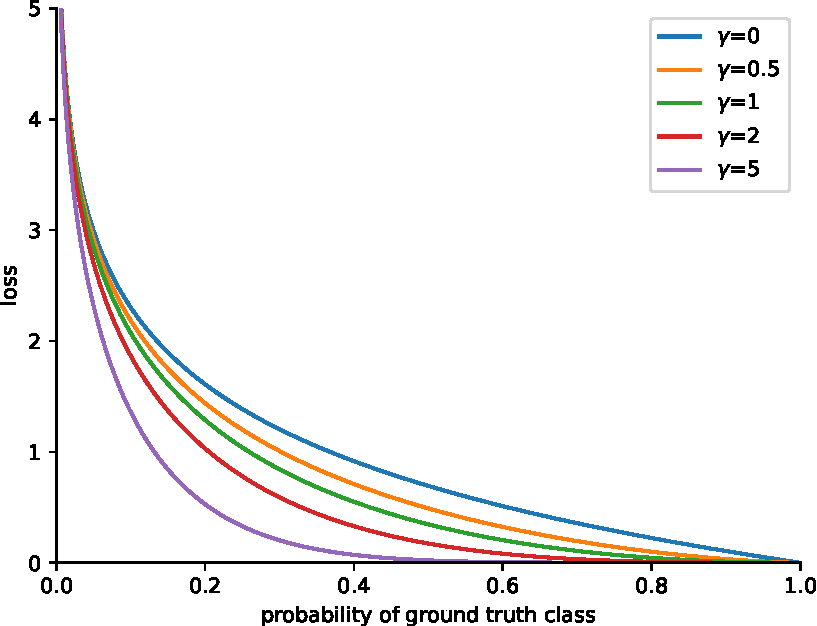
\includegraphics[width=0.5\textwidth]{figures/ch3/fig3.pdf}
  \caption{Well classified examples, ($p\geq0.6$) contribute to the overall much less than hard examples. For $\gamma=0$, focal loss equals to the cross-entropy loss.}
  \label{ch3:fig3}
\end{figure} 

\section{RetinaNet}
RetinaNet was introduced as a single-stage adaptation of the Feature Pyramids Networks (FPN, \cite{lin2017feature}) with the enhancement of focal loss. It is the bridge between double-stage and single-stage detection, as it surpassed the performance of Faster R-CNN with detection rates similar to YOLO and SSD.

Detecting objects at different scales is a demanding task, and the standard approach is using image pyramids. SSD made one of the first attempts in multi-scale object detection by exploiting network's pyramidal feature hierarchy. Feature maps from deeper layers are semantically stronger than those from shallower levels of the convolutional network. This pyramidal information hierarchy results in feature maps large in spatial size but weak in information, and in coarse feature maps with high levels of information. RetinaNet exploits this hierarchy by combining spatially large but semantically weak maps with coarser, semantically stronger, activation maps.

\begin{figure}[!htb]
  \centering
  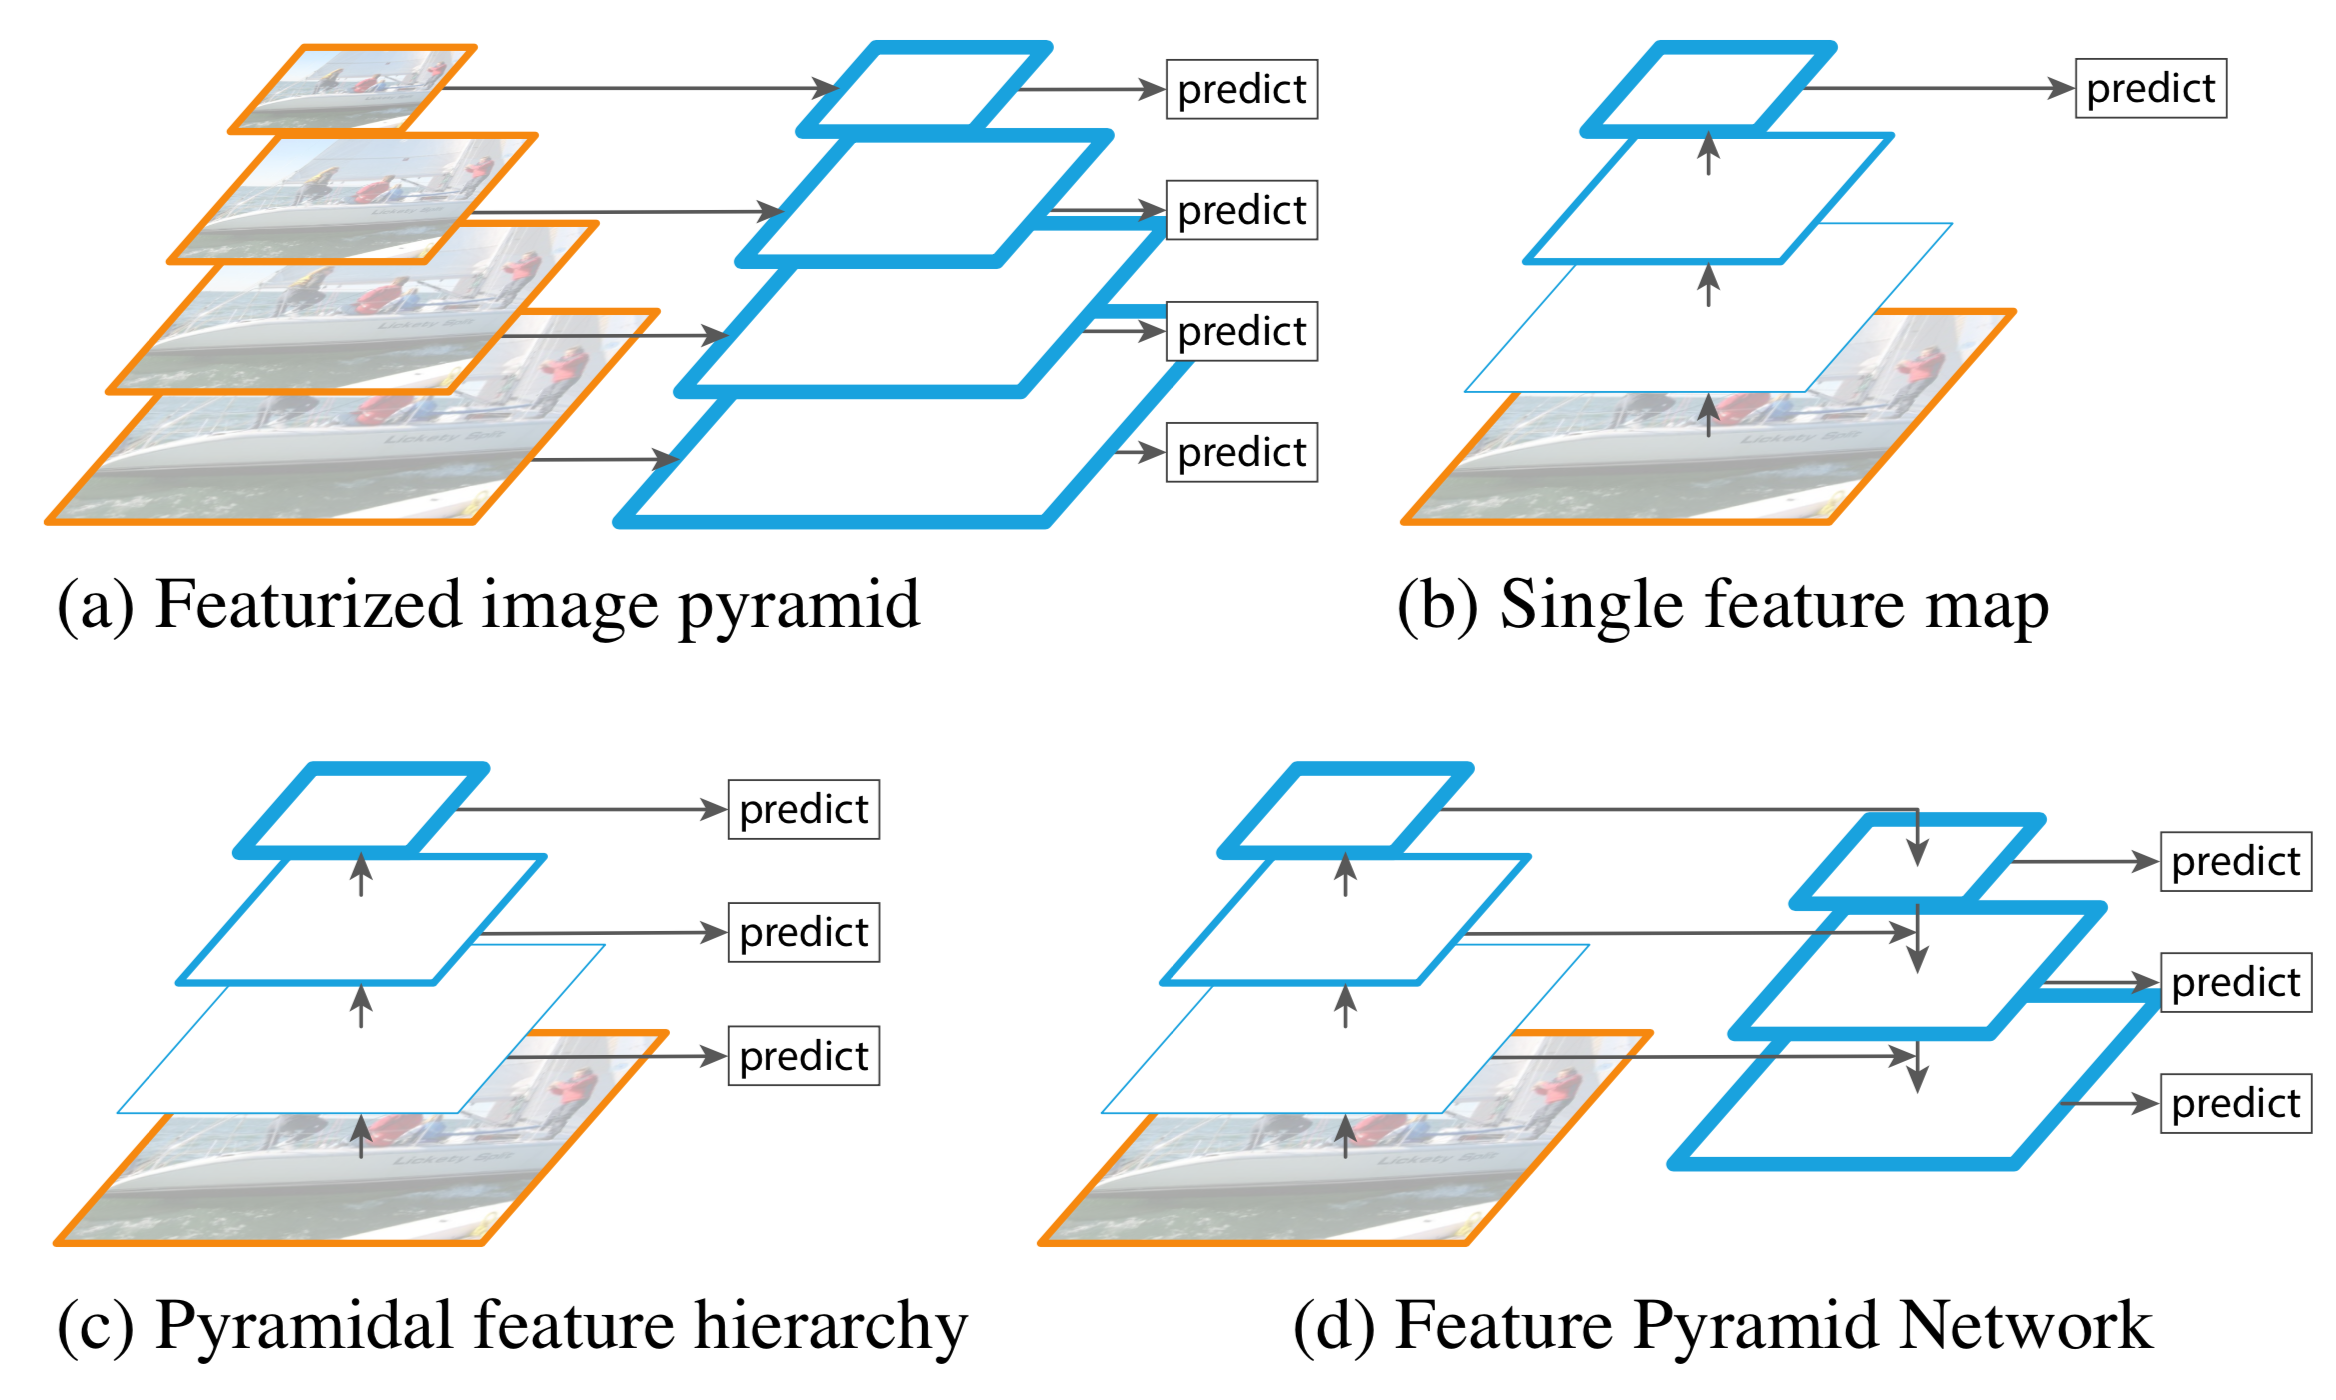
\includegraphics[width=12cm]{figures/ch3/fig4.png}
  \caption{Different types of pyramidal feature exploitation. Reproduced from \cite{lin2017feature}}
  \label{ch3:fig4}
\end{figure} 

\fref{ch3:fig4} shows different types of pyramidal feature exploitation: (a) Building an image pyramid by feeding an image in multiple scales. It used to be a common practice, but it is computationally infeasible. (b) Feeding an image and making predictions from the coarsest, rich in information, feature map. It is a fast method for making single scale predictions (as seen in the first version of YOLO). (c) Detection in different scales by exploiting feature maps in the intermediate layers (mainly adopted by the SSD). (d) The FPN method. Detects objects at different scales as the standard SSD detector, but layers are semantically enriched from the deeper layers via the top-down path.

\subsection{Architecture}
\fref{ch3:fig5} illustrates the main pipeline of the Feature Pyramid Network that was adopted by the RetinaNet. During the bottom-up pathway, the backbone network computes feature maps at several scales with the help of pooling operations. In the case of the VGG architecture, the backbone consists of 5 convolutional blocks where each one of them produces feature maps downscaled by a factor of 2, resulting in the features $(C_1, C_2, C_3, C_4, C_5)$. During the top-down pathway, the feature maps $C_i$ are obtained via lateral connections and convolved with $1\times1$ kernels to reduce their depth, preserving their spatial size. Then, each feature map is upsampled, by the nearest neighbour method, and it is added element-wise to the $C_{i}$ reduced map of the previous layer. Finally, the aliasing effect of each merged map, due to upsampling is reduced by a final $3\times3$ convolution. The result is a set of features $(P_1,P_2,P_3,P_4,P_5)$, where each $P_i$ contains information from the deeper layer features $C_{j\geq i}$. 

\begin{figure}[!htb]
  \centering
  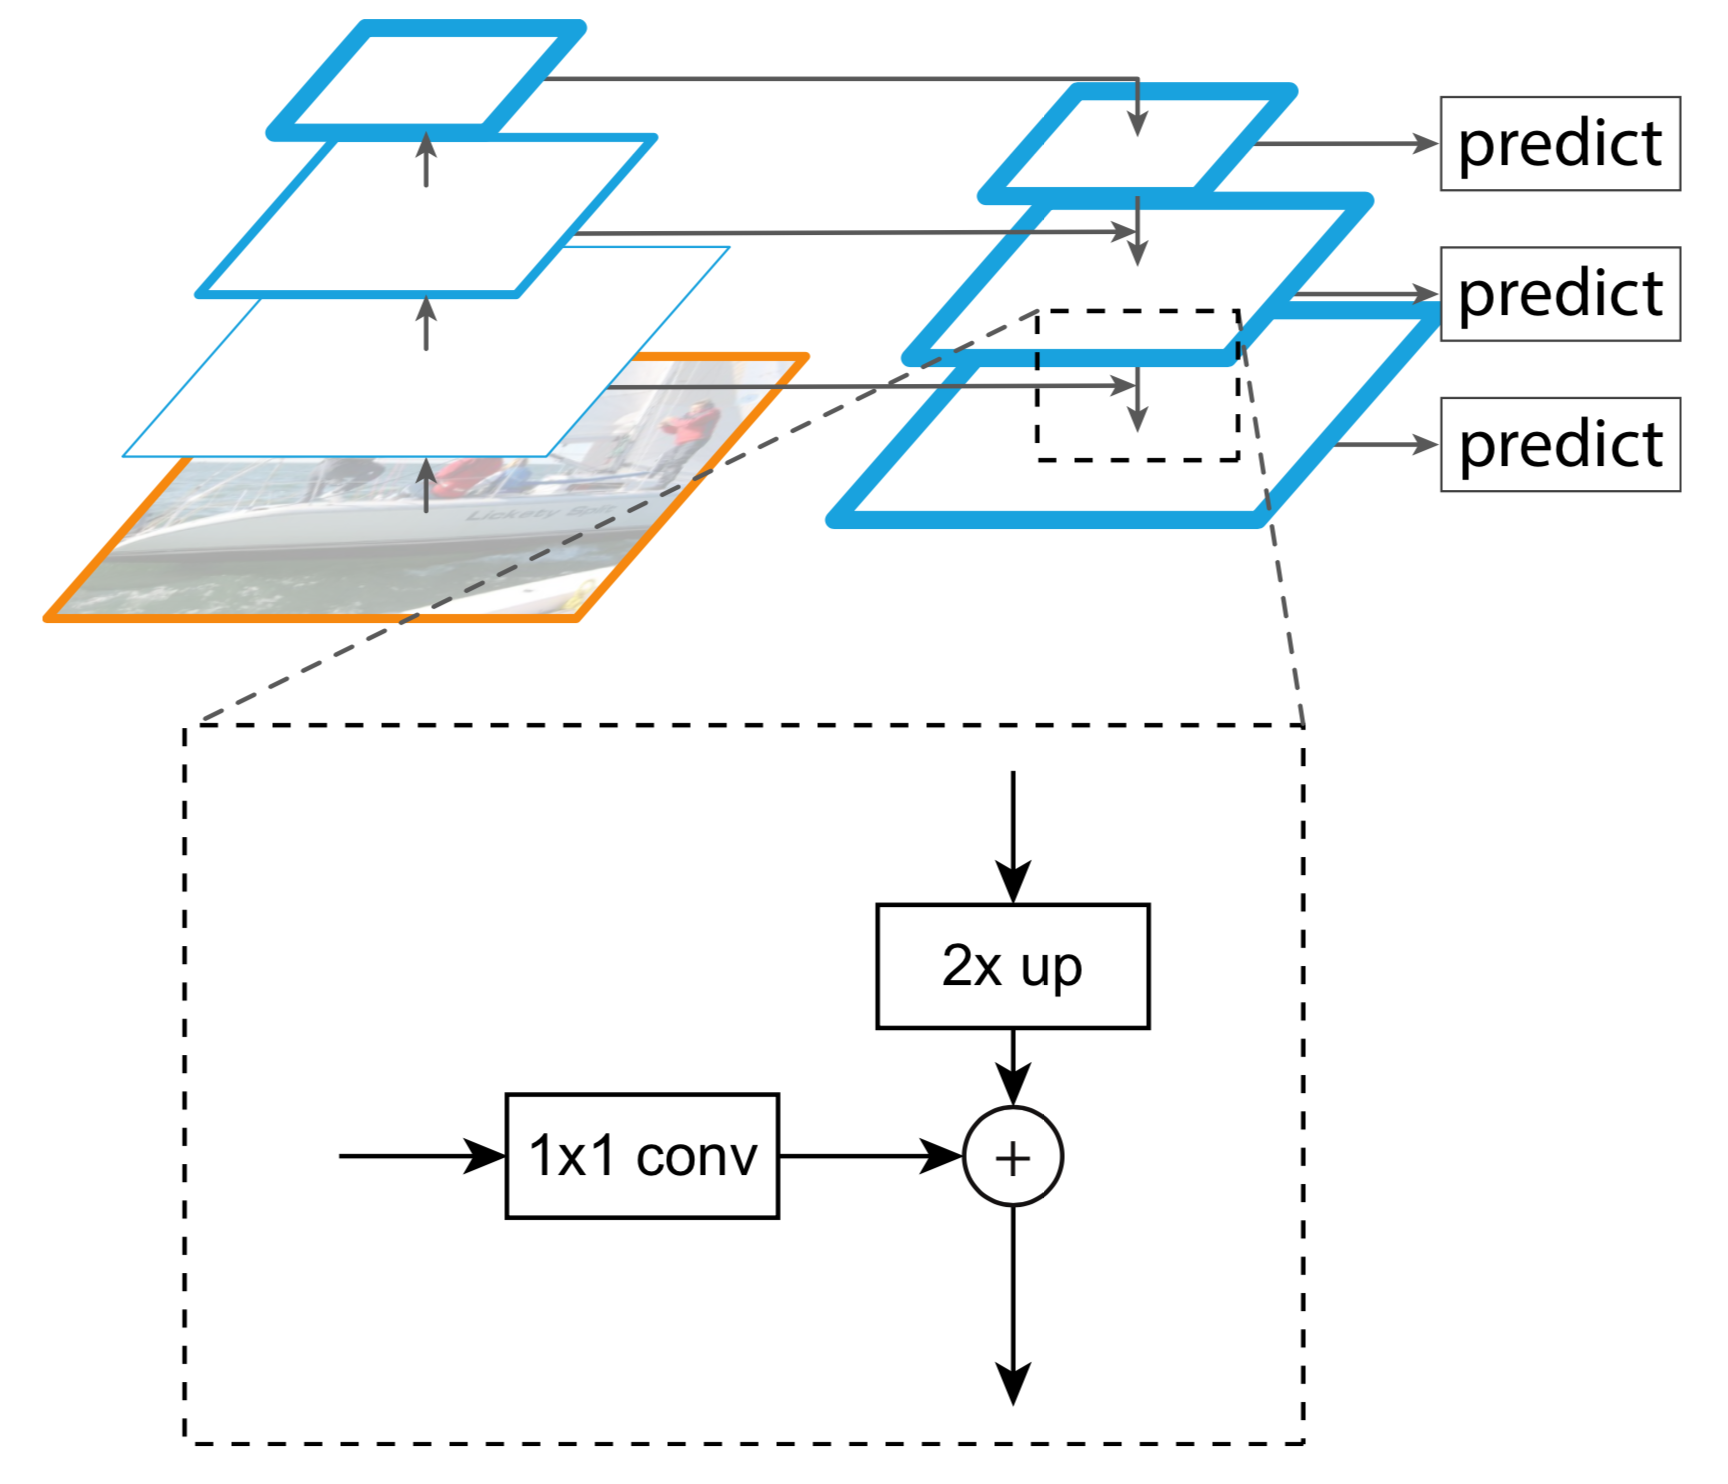
\includegraphics[width=6cm]{figures/ch3/fig5.png}
  \caption{The top-down building block in RetinaNet and FPN. Reproduced from \cite{lin2017feature}.}
  \label{ch3:fig5}
\end{figure} 

In fact, instead of featurising the output layers in each convolutional block, RetinaNet attaches at the end of the backbone network two more $3\times3$ strided convolutional layers, continuing downscaling by the same factor the output, without making use of pooling. These outputs are noted as $C_6,C_7$ and the featurised levels are the set $(C_3, C_4, C_5, C_6, C_7)$ which produce the output pyramidal layers $(P_3, P_4, P_5, P_6, P_7)$. The pipeline of RetinaNet can be seen in \fref{ch4:fig3}.

\subsection{Anchor Boxes}
RetinaNet adopts the anchor boxes concept to produce RoIs, in contrast with the FPN which uses a region proposal network. Due to the number of pooling operations every pyramidal level has undergone, the stride in each $P_i$ layer is $(8, 16, 32, 64, 128)$\footnote{$P_3$ has already been pooled 3 times from block$_1$, block$_2$ and block$_3$, thus it has a stride of $2^3$.}. The effective receptive field of each layer is crucial since it acts as a limiting factor for the size of the anchors and the size of the detected object as a consequence; stride, on the other hand, indicates the density of the predictions (as discussed in \sref{anchor_box}). However, in RetinaNet, this is not completely true as each $P_i$ is the product of many layer outputs, from various depths with different receptive fields and different levels of information. In general, spatially large $P_i$ features aim in dense small object detection, while coarser $P_i$ maps are responsible for large object detection. Specifically, each layer's anchors have three scales and three ratios. Anchor's base size is $(32^2, 64^2, 128^2, 256^2, 512^2)$ with scales $(2^0, 2^{1/3}, 2^{2/3})$ and ratios of $(1\!:\!2,1\!:\!1,2\!:\!1)$.

\subsection{Prediction Subnet}
The subnetwork responsible for detections consists of a classification and a box regression subnet. The classification subnet consists of 4 stacked $3\times3\times C$ convolutional kernels with ReLU activations, followed by a $3\times3\times KA$ filter with sigmoid activation and predicts a $p(c_i)$, out of K classes, for each anchor. C is the channel depth of each $P_i$ and it is the same for all layers.

The class agnostic box regression subnet follows the same logic with 4 stacked $3\times3\times C$ convolutional kernels with ReLU activations, followed by a $3\times3\times 4A$ filter with sigmoid activation. The output is a four-tuple, containing each anchor's refined coordinates. The prediction subnet shares its parameters across all pyramidal $P_i$ outputs, following SSD's philosophy.

\section{Evaluation Metrics}
Object detection has several evaluation metrics; nevertheless, performance comparisons depend on the problem. For example, in the PASCAL-VOC challenge, models compete between those with the highest mAP, while in the fruit detection problem, higher F1-score is more desirable. However, the most useful metrics are:

\bigskip
\textbf{Recall}
\bigskip\noindent
\begin{equation}
  \text{Recall} = \frac{TP}{TP+FN}=\frac{TP}{\text{Num. of objects}}
\end{equation} 

The Recall is the fraction between the successfully detected instances and the total number of instances. A true positive is considered as positive if its bounding box has an IoU with the ground truth annotation, above a certain threshold. Usually, this threshold is set at 0.5.

\bigskip
\textbf{Precision}
\bigskip\noindent
\begin{equation}
  \text{Precision} = \frac{TP}{TP+FP}=\frac{TP}{\text{Predictions}}
\end{equation} 

Precision gives the ability of the model identifying only the relevant instances as it gets lower for every wrong prediction.

\bigskip
\textbf{F1-score}
\bigskip\noindent
\begin{equation}
  \text{F1-score} = 2\times\frac{\text{Precision}\times \text{Recall}}{\text{Precision}+\text{Recall}}\end{equation} 
  
The F1-score is the harmonic mean between precision and recall, giving equal importance in both. It is used, mostly in tasks where the model should have the best ratio between true positives and false positives. A change in the detector's confidence threshold comes with an expense in the rate of true positives along with the rate of false positives. Increasing detector's confidence threshold reduces false positives and true positives at the same time, while decreasing it has the opposite effect. F1-score indicates the point in the precision-recall curve, where precision and recall have similar maximum values.

\bigskip
\textbf{Average Precision}
\bigskip\noindent

Average precision (AP) is the area under the precision-recall curve (AUC). The PR curve usually follows a zigzag pattern complicating its calculation. \cite{everingham2010pascal} proposed a widely adopted method to calculate the AUC by interpolating precision in 11 evenly spaced points. The precision at each recall level takes the maximum value in order to eliminate this zigzag pattern.

\begin{align}
  \text{AP} &= \frac{1}{11}\sum_{r\in\{0,0.1,...,1\}}p_{interp}(r)	&	p_{interp}(r) &= \max_{\tilde{r}:\tilde{r}\geq p(\tilde{r})}
\end{align} 

In this study, the primary evaluation metric is the F1-score, along with other secondary metrics such as the AP, and the mean IoU between predictions and true positives. For the apple counting task, the only metric is the relative error between the number of predictions and the total number of instances in the dataset.